\chapter{Methodology}
\label{chap:methodology}

In this chapter, we describe the key models and functions utilized in our approach. Each model is carefully selected based on its capabilities and suitability for solving the specific challenges presented by our task.

\section{Models Used}

\subsection{YOLOS}

YOLOS (You Only Look One-level Series) is a Vision Transformer (ViT) based object detection model developed to reframe object detection as a direct prediction problem, without relying on anchors or region proposals. It employs a pure transformer encoder architecture to predict object bounding boxes and their associated classes in a single forward pass.

In our project, we fine-tuned a YOLOS model using the Fashionpedia dataset. The model was trained to detect bounding boxes around clothing items in images. For instance, when presented with a celebrity image, the fine-tuned YOLOS model identifies the various garments (such as shirts, pants, or dresses) worn by the individual and provides the corresponding bounding boxes and class labels.

Once a clothing item (e.g., a shirt) is detected, we crop the region inside the bounding box and use it as input for downstream retrieval tasks using FashionCLIP.

\textbf{Justification:} YOLOS was chosen because of its simplicity and effectiveness in object detection tasks without relying on complex region proposal networks. Its transformer-based architecture aligns well with modern deep learning trends and has shown competitive performance on several benchmarks. By fine-tuning YOLOS on the Fashionpedia dataset, we ensured that the model is well-adapted to the specific visual characteristics and labeling conventions present in fashion imagery.

\subsection{FashionCLIP}

FashionCLIP is a domain-specific adaptation of the original CLIP model, fine-tuned on a large corpus of fashion-related images and textual descriptions. It leverages a ViT-B/32 Transformer as the image encoder and a masked self-attention Transformer for text encoding. The two modalities are trained jointly using a contrastive loss to maximize the similarity between corresponding (image, text) pairs.

FashionCLIP, as CLIP, creates a shared vector space for images and text. This allows us to tackle many tasks, such as retrieval (find the image that is most similar to a given query).

\begin{figure}[H]
\centering
  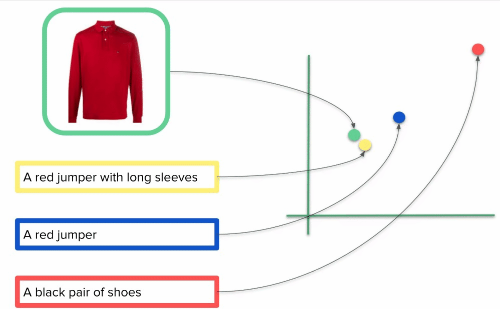
\includegraphics[width=0.5\textwidth]{images/shared-vs.png}
\end{figure}


There are basically two main components, and image encoder (to generate a vector starting from an image) and a text encoder (to generate a vector starting from a piece of text). The two encoders are trained together, so that the image and text encoders are aligned in the same vector space. This means that if you have an image and a piece of text that describe the same thing, their vectors will be close to each other in this space. A rough visualization of this is shown in Figure below.

\begin{figure}[H]
  \centering
      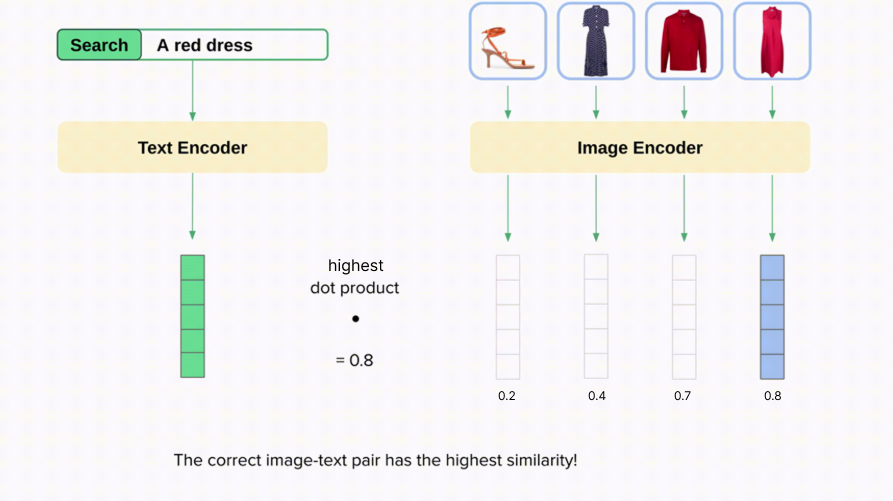
\includegraphics[width=0.6\textwidth]{images/dotprod.png}
  \end{figure}

The similarity between an image and a text, or between two images (or texts) can be calculated using the cosine similarity formula:

  \[
  \text{Similarity}(\mathbf{I}, \mathbf{T}) = \frac{\mathbf{I} \cdot \mathbf{T}}{\|\mathbf{I}\| \|\mathbf{T}\|}
  \]

  Where:

  \begin{itemize}
    \setlength\itemsep{-1.5em}
      \item $\mathbf{I}$ is the embedding vector for the image.
      \item $\mathbf{T}$ is the embedding vector for the text.
      \item $\cdot$ denotes the dot product between the image and text embeddings.
      \item $\|\mathbf{I}\|$ and $\|\mathbf{T}\|$ are the magnitudes (or norms) of the image and text vectors, respectively, used to normalize the dot product.
  \end{itemize}

  This equation calculates the cosine similarity between the image and text embeddings, which measures how closely related they are in the shared vector space created by FashionCLIP.

In our project, FashionCLIP is used to generate embeddings for both inventory images and their textual descriptions. These embeddings are stored in a FAISS database for efficient similarity search. At query time, a user can either input an image (e.g., cropped garment detected by YOLOS) or text (e.g., ``red summer dress''), which is embedded using FashionCLIP and matched against the inventory to find the closest fashion items.

\textbf{Justification:} FashionCLIP was specifically selected due to its fine-tuning on a dedicated fashion dataset, which makes it exceptionally good at capturing the nuances and semantics of fashion-related queries. Unlike the general CLIP model, FashionCLIP is better suited to the unique distribution of fashion imagery and descriptions, enabling more accurate and meaningful retrieval results in our inventory search use case. Its flexibility in handling both text and image queries makes it an ideal choice for a multimodal search system.

\section{Functions Used}

In this section, we describe the custom utility functions implemented to support data preprocessing, transformation, visualization, and model training.

\subsection*{fix\_channels}
This function standardizes the number of image channels to three. It handles cases where images have a single grayscale channel or four channels (with transparency) by converting them into standard three-channel RGB images.

\vspace{-1.25em}
\subsection*{xyxy\_to\_xcycwh}
Converts bounding box coordinates from (top-left and bottom-right corners) format $(x_1, y_1, x_2, y_2)$ into (center x, center y, width, height) format, which is often preferred for training object detection models.

\vspace{-1.25em}
\subsection*{cxcywh\_to\_xyxy}
Performs the inverse operation of \texttt{xyxy\_to\_xcycwh}, converting bounding boxes from center coordinates and size back to corner coordinates.

\vspace{-1.25em}
\subsection*{rescale\_bboxes}
Handles the normalization and denormalization of bounding boxes. It scales bounding box coordinates between absolute pixel values and relative values in the range [0, 1], depending on the model or visualization requirements.

\vspace{-1.25em}
\subsection*{plot\_results}
A visualization function that draws predicted bounding boxes on top of images. It also annotates each box with the predicted category label, using predefined colors for better readability.

\vspace{-1.25em}
\subsection*{idx\_to\_text}
Maps category indices to their corresponding human-readable category names based on the dataset's class definitions.

\vspace{-1.25em}
\subsection*{filter\_invalid\_bboxes}
Filters out invalid bounding boxes where coordinates do not form a valid rectangle. This helps ensure that only correctly defined objects are used during training and evaluation.

\vspace{-1.25em}
\subsection*{transform}
Prepares input batches for model training or inference. It processes images and annotations, fixes channels, rescales bounding boxes, converts bounding box formats, and packages everything into the required structure for model input.

\vspace{-1.25em}
\subsection*{transform\_train and transform\_val}
Simple wrappers around the \texttt{transform} function, used to differentiate preprocessing pipelines between training and validation phases if needed.

\vspace{-1.25em}
\subsection*{draw\_augmented\_image\_from\_idx}
Draws an annotated image sample from the dataset, optionally applying transformations (such as augmentations) before visualization. Useful for inspecting dataset quality or augmentation effects.

\vspace{-1.25em}
\subsection*{plot\_augmented\_images}
Plots multiple samples from the dataset in a grid layout. It uses \texttt{draw\_augmented\_image\_from\_idx} internally and helps visualize a batch of images along with their annotations.

\vspace{-1.25em}
\subsection*{Detr Class}
A PyTorch Lightning module encapsulating the YOLOS model for training and validation. It implements common deep learning utilities like optimizer configuration, loss computation, and data loading.

\vspace{-1.25em}
\subsection*{get\_text\_based\_rec}
Given a textual query, this function uses FashionCLIP to encode the text into an embedding, computes similarity scores against precomputed image embeddings, and retrieves the top-$k$ most similar products.

\vspace{-1.25em}
\subsection*{get\_image\_based\_rec}
Takes an input image, encodes it into an embedding using FashionCLIP, searches the FAISS image index for the top-$k$ nearest neighbors, and returns the corresponding product identifiers.

